% vim: set tw=0:
\documentclass{beamer}
\usepackage{graphicx}
\usepackage{hyperref}
\hypersetup{pdfborder={0 0 0 0}}

% Reasonable themes:
% Antibes Bergen Berkeley Berlin Frankfurt Goettingen Ilmenau Luebeck Malmoe
% Montpellier PaloAlto Rochester Singapore Szeged Warsaw bars boxes
% compatibility default lined plain shadow sidebar split tree
% And these ones include the author's name on every slide:
% Berkeley

% Declare themes.
\mode<presentation>
\usetheme{UWHEP}

% Personal macros.
\newcommand{\email}[1]{{\texttt #1}}
\newcommand{\newframe}[1]{\section{#1}
    \frametitle{\sc{#1}}}
\newcommand{\subframe}[1]{\subsection{#1}
    \frametitle{\sc{#1}}}
\newcommand{\supers}[1]{\ensuremath{^\textrm{#1}}}
\newcommand{\subs}[1]{\ensuremath{_\textrm{#1}}}
\newcommand{\ca}{\ensuremath{\sim}}
\renewcommand{\email}[1]{\href{mailto:#1}{\nolinkurl{#1}}}

% Author information.
\title{Storage at UW-Madison CMS Tier-2}
\author[Maier]{
    Will Maier \\ 
    {\tt wcmaier@hep.wisc.edu}}
\institute[Wisconsin]{University of Wisconsin - High Energy Physics}
\date[2010.09.22]{OSG Storage Forum, U. Chicago}
\logo{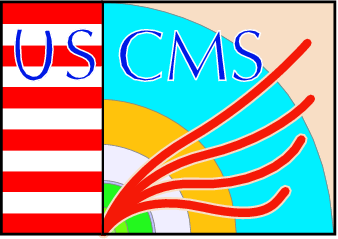
\includegraphics[height=0.6cm]{../../Graphics/USCMS_logo.png}\hspace{.1cm}
\includegraphics[height=0.75cm]{../../Graphics/UW_logo.png}}

\begin{document}

% http://indico.fnal.gov/conferenceTimeTable.py?confId=3377
% 15 min
% hardware/layout
% software
% monitoring/management
% evaluation
% plans

\begin{frame}
    \titlepage
\end{frame}

\section{Overview}
\begin{frame}
    \tableofcontents
\end{frame}

\section{Hardware}
\subsection{Core}
\begin{frame}
\begin{itemize}
	\item Four core dCache machines: PNFS, admin/misc, doors, hotspare
	\item 1 Gbps connections, SATA disks, 2x2 2.0 GHz Opterons, 16 GB RAM
	\item PNFS: RAID10 (10kRPM disks), 2x4 3.0 GHz Xeons
	\begin{itemize}
		\item Current configuration \ca{}12 months old
		\item Nearly saturated (again)\ldots{}need more IO
	\end{itemize}
	\item admin, doors, hotspare: commodity, nothing special
	\begin{itemize}
		\item No observed scaling issues with shared SRM/dcap door
		\item \ca{}32 GridFTP doors live on data nodes (easy to add more)
	\end{itemize}
	% plot requests/time? files?
\end{itemize}
\end{frame}

\subsection{Cluster}
\begin{frame}
\begin{itemize}
	\item \ca{}50\% dedicated, \ca{}50\% shared with compute resources
	\item Dedicated nodes: mix of RAID6, RAID0 with 1 - 2 TB SATA disks
	\item Shared nodes: no RAID, .5 - 2 TB SATA disks (4 - 16 slots, 2 - 48 GB RAM)
	\item 908(ish) pools on 210 nodes (one pool per disk, mostly)
	\item Redundant 2x10 Gbps network (and several stacks of Cisco 3750s) managed by campus
	% XXX: plot: TB/time
\end{itemize}
\end{frame}

\section{Management}
\subsection{Administration} % cli, dcache_tools, dcache info provider
\begin{frame}
\begin{itemize}
	\item Install nodes with kickstart, manage live configuration with Cfengine (v2)
	\item Management scripts written with dcache-tools~\footnote{\url{http://code.hep.wisc.edu/dcache-tools}}, based on CLI~\footnote{\url{http://packages.python.org/pyCLI}}
	\begin{itemize}
		\item {\tt dcache\_absent}: List absent and offline pools
		\item {\tt dcache\_billingrep}: Watch billing log and initiate replications of new files
		\item {\tt dcache\_clean}: Remove invalid/unlinked files directly from pools
		\item {\tt dcache\_df}: {\tt df(1)}-like overview of cluster storage
		\item etc\ldots{}
	\end{itemize}
	\item Less web scraping, more dCache info provider
	\begin{itemize}
		\item Previously, most monitors/checks polled dCache web pages and scraped HTML
		\item Info provider allows simple XML parsing (and exposes lots of detail)
		\item Can request subsets of data (ie for {\tt dcache\_df})
	\end{itemize}
\end{itemize}
\end{frame}

\subsection{Alerts and Trends} % nagios
\begin{frame}
\begin{itemize}
	\item Nagios checks for all servers in both the core and cluster
	\item Some Nagios protocol checks (GridFTP, SSH admin interface)
	\item Functional tests via cron jobs (SRM/dcap/GridFTP read/write)
	\item External monitoring (CMS SAM, JobRobot, Dashboard, SiteView, PhEDEx; OSG RSV, MyOSG, Gratia; \ldots{})
	\item Aggregate local monitoring in tsar~\footnote{\url{http://code.hep.wisc.edu/tsar}}
	\begin{itemize}
		\item Ingest time series data from simple collectors
		\item Supports HTTP, other submission/query protocols to come
		\item Data in memory for fast writes/reads (Redis~\footnote{\url{http://redis.io}} backend)
		\item JavaScript, Python clients for visualization~\footnote{\url{http://tsar.hep.wisc.edu/plots/dcache}}
	\end{itemize}
\end{itemize}
\end{frame}

\section{Evaluation}
\subsection{What Works}
\begin{frame}
\begin{itemize}
	\item Co-locating storage and compute services on commodity hardware
	\item Close network collaboration with University
	\item dCache (stability, throughput)
	\item Increasingly centralized monitoring and reporting
\end{itemize}
\end{frame}

\subsection{What Doesn't}
% dcache hotspots
\begin{frame}
\begin{itemize}
	\item Monitoring fragmentation
	\item dCache (hotspots, replication, commodity data servers)
	\item Disks
	\item VDT (for us, with caveats)
\end{itemize}
\end{frame}

\section{Plans}
\begin{frame}
\begin{itemize}
	\item Centralize dCache logging
	\item Scale tsar
	\item Transition to alerting based on trends (instead of binary checks)
	\item Explore HDFS w/ xrootd frontend (to support jobs on local opportunistic resources)
	\item PNFS $\rightarrow$ Chimera? dCache $\rightarrow$ HDFS?
	\item Cfengine 2 $\rightarrow$ Cfengine 3/Puppet/Chef/\ldots{}?
	\item Expand use of RPMs (for improved atomicity?)
\end{itemize}
\end{frame}

\end{document}
